\documentclass[10pt,a4paper]{article}
\usepackage[utf8]{inputenc}
\usepackage{graphicx}
\def\Pr{\mathop{\rm Pr}}
\usepackage[landscape,margin=1cm]{geometry}
\usepackage[english]{babel}
\usepackage{hyperref}
\hypersetup{
    colorlinks=true,
    linkcolor=blue,
    filecolor=magenta,      
    urlcolor=blue,
}

\usepackage{multicol}
% colour themes to come. KnitR?

%-------------------------

\title{Probability and Statistical Inference}
\author{John S Butler }
%\date{July 2019}
\usepackage[default]{raleway}
\usepackage{fontawesome}
\usepackage[T1]{fontenc}

\usepackage{hyperref}
\usepackage{enumitem}
\usepackage{lipsum}

\usepackage{xcolor}
\definecolor{customcolor}{HTML}{616AC5}
\definecolor{alert}{HTML}{CD5C5C}
\definecolor{w3schools}{HTML}{4CAF50}
\definecolor{subbox}{gray}{0.60}
\definecolor{codecolor}{HTML}{FFC300}
\colorlet{xx}{customcolor}


%--------------------------Editor mode.

\usepackage
[citestyle=authoryear,
sorting=nty,	  		%Sorts bibliography by year, name, title
autocite=footnote, 		%Autocite command generates footnotes
autolang=hyphen, 		
mincrossrefs=1, 	
backend=biber]
{biblatex}

\DeclareFieldFormat{postnote}{#1}
\DeclareFieldFormat{multipostnote}{#1}
\DeclareAutoCiteCommand{footnote}[f]{\footcite}{\footcites}

\bibliography{literature}
%----------------------------------------
%--------------------------------------------------------------------------------
\usepackage{tcolorbox}

\tcbuselibrary{most,listingsutf8,minted}

\tcbset{tcbox width=auto,left=1mm,top=1mm,bottom=1mm,
right=1mm,boxsep=1mm,middle=1pt}

\newenvironment{mycolorbox}[2]{%
\begin{tcolorbox}[grow to left by=-1em,grow to right by=-1em,capture=minipage,fonttitle=\large\bfseries, enhanced jigsaw,boxsep=1mm,colback=#1!30!white,on line,tcbox width=auto, toptitle=0mm,colframe=#1,opacityback=0.7,nobeforeafter,title=#2]%
}{\end{tcolorbox}\\[0.2em]}

\newenvironment{subbox}[2]{%
\begin{tcolorbox}[capture=minipage,fonttitle=\normalsize\bfseries, enhanced jigsaw,boxsep=1mm,colback=#1!30!white,on line,tcbox width=auto,left=0.3em,top=1mm, toptitle=0mm,colframe=#1,opacityback=0.7,nobeforeafter,title=#2]\footnotesize %
}{\normalsize\end{tcolorbox}\vspace{0.1em}}

\newenvironment{multibox}[1]{%
\begin{tcbraster}[raster columns=#1,raster equal height,nobeforeafter,raster column skip=1em,raster left skip=1em,raster right skip=1em]}{\end{tcbraster}}

\newenvironment{textbox}[1]{\begin{mycolorbox}{customcolor}{#1}}{\end{mycolorbox}}

%-------------------------------
\newtcblisting{codebox}[2]{colback=codecolor!5,colframe=codecolor!80!black,listing only, 
minted options={numbers=left,style=tcblatex,fontsize=\tiny,breaklines,autogobble,linenos,numbersep=3mm},
left=5mm,enhanced,
title=#2, fonttitle=\bfseries,
listing engine=minted,minted language=#1}

%--------------------------------------------------------------------------------
\newcommand{\punkti}{~\lbrack\dots\rbrack~}

\renewenvironment{quote}
               {\list{\faQuoteLeft\phantom{ }}{\rightmargin\leftmargin}%
                \item\relax\scriptsize\ignorespaces}
               {\unskip\unskip\phantom{xx}\faQuoteRight\endlist}
               

%--------------------------------------------------------------------------------
\newcommand{\bgupper}[3]{\colorbox{#1}{\color{#2}\huge\bfseries\MakeUppercase{#3}}}
\newcommand{\bg}[3]{\colorbox{#1}{\bfseries\color{#2}#3}}

\newcommand{\mycommand}[2]{{\ttfamily\detokenize{#1}}~\dotfill{}~{\footnotesize #2}\\}
\newcommand{\sep}{{\scriptsize~\faCircle{ }~}}


\newcommand{\bggreen}[1]{\medskip\bgupper{w3schools}{black}{#1}\\[0.5em]}
\newcommand{\green}[1]{\smallskip\bg{w3schools}{white}{#1}\\}
\newcommand{\red}[1]{\smallskip\bg{alert}{white}{#1}\\}

\usepackage{multicol}
\setlength{\columnsep}{30pt}

\setlength{\parindent}{0pt}
\pagestyle{empty}

\usepackage{csquotes}

\newcommand{\loremipsum}{Lorem ipsum dolor sit amet.}



%--------------------------------------------------------------------------------
\begin{document}
\small
\begin{multicols}{3}

%\maketitle
%\thispagestyle{empty}
\scriptsize
%\tableofcontents


%\section{Data Type}
\section*{Probability and Statistical Inference}
\subsection*{Cheat Sheet}
%\href{https://sites.google.com/dit.ie/math4001
%}{Course} Cheat Sheet}

\subsubsection*{\href{johnsbutler.netlify.com}{John S Butler} (TU Dublin) }
\subsubsection*{\href{https://twitter.com/StatisticalInf1}{Course Twitter Account} }
\begin{textbox}{Data Type}
\begin{multicols}{2}
\begin{itemize}
  \item Categorical
  \item Interval
  \item Ordinal
  \item Ratio
\end{itemize}

\end{multicols}

\end{textbox}


\begin{textbox}{Measures of Location}
Different aspects of a distribution of data can be summarised by the measures of location:
\begin{enumerate}
    \item The First Moment: Mean, Mode or Median;
    \item  The Second Moment: Variance, Standard Deviation;
    \item  The Third Moment: Skewness.
\end{enumerate}

\begin{subbox}{subbox}{First Moment: Middle}
\begin{center}
\tiny
    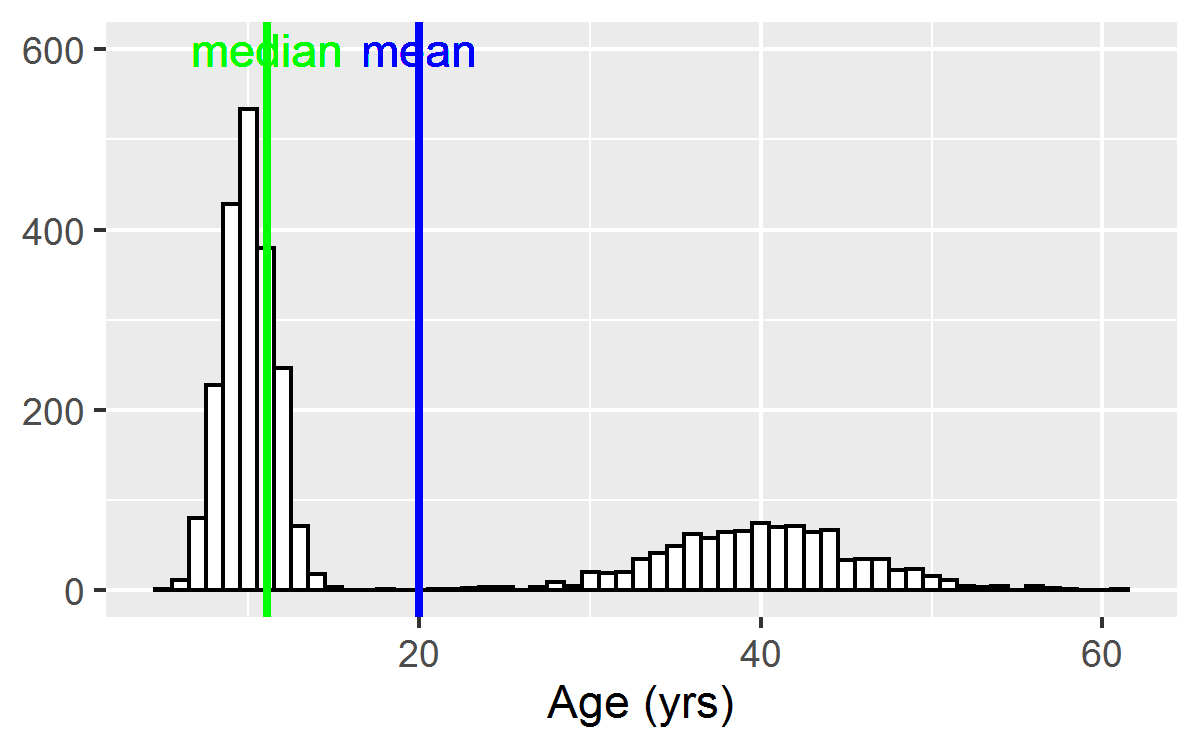
\includegraphics[width=\textwidth]{Figures/Measures_of_Location/middle.png}
\end{center}

\end{subbox}

\begin{subbox}{subbox}{Second Moment: Spread}
\begin{center}
\tiny
    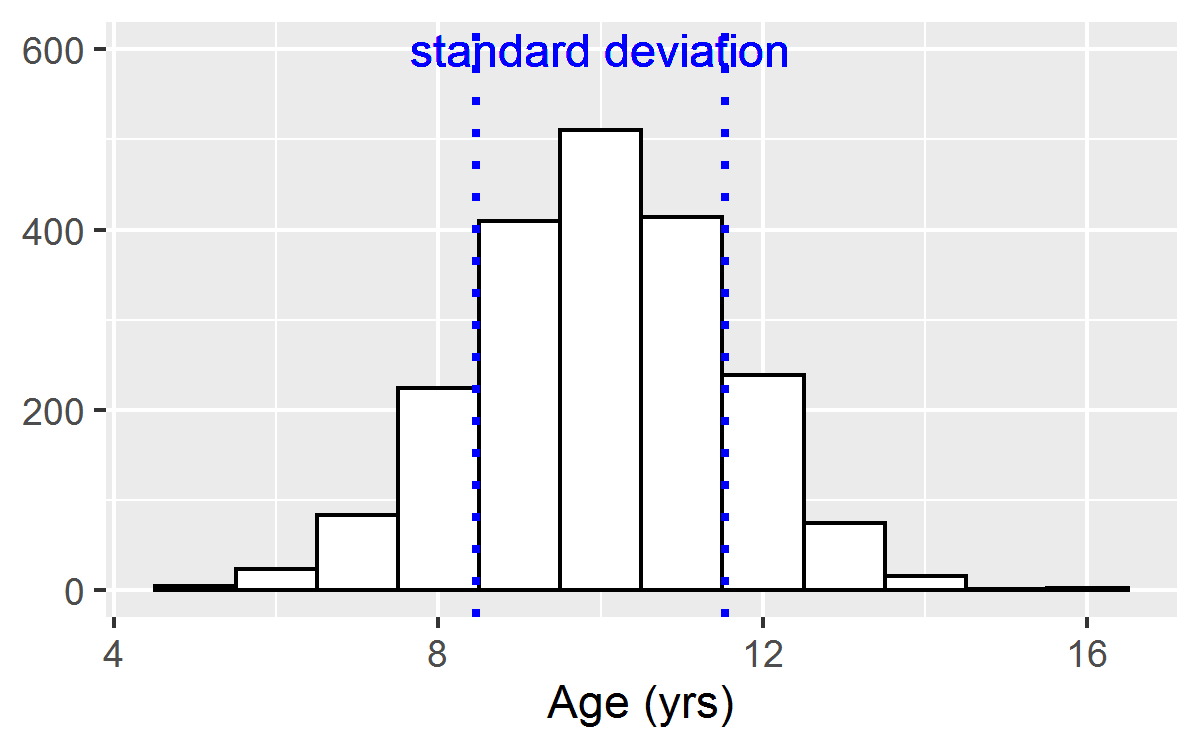
\includegraphics[width=\textwidth]{Figures/Measures_of_Location/range.png}
\end{center}

\end{subbox}
\end{textbox}
%% NEW TEXT BOX MEASURES OF LOCATION
\begin{textbox}{Measures of Location (cont.)}

\begin{subbox}{subbox}{Third Moment: Symmetry}
\begin{center}
\tiny
    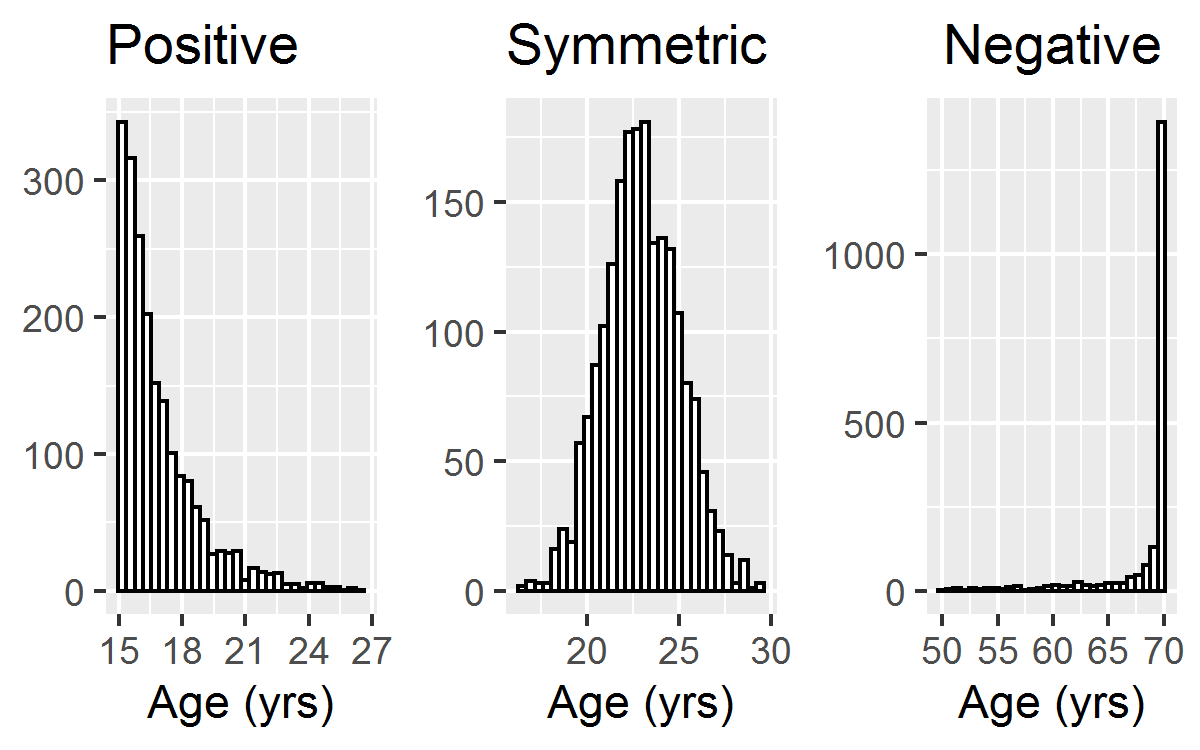
\includegraphics[width=\textwidth]{Figures/Measures_of_Location/skew.png}
  
    
\end{center}
\end{subbox}
\end{textbox}
\begin{textbox}{Mathematical Probability }
\begin{subbox}{subbox}{Definitions}
\tiny
Define some event $A$ that can be the outcome of an experiment.\\
$\Pr(A)$ is the probability of a given event $A$ will happen.\\
Rules:
\begin{itemize}
    \item $\Pr(A)$ is between $0$ and $1$, $0\leq Pr(A) \leq 1$;
    \item $\Pr(A)=1$, means it will definitely happen;
    \item $\Pr(A)=0$, means it will definitely \textbf{not} happen;
    \item $\Pr(A)=0.05$, is arbitrarily considered unlikely.
\end{itemize}
\end{subbox}

\begin{subbox}{subbox}{Sample Space and Events}
\tiny
The \textbf{Sample Space}, $S$, of an experiment is the universal set of all possible outcomes for that experiment, defined so, no two outcomes can occur simultaneously. For example:
\begin{itemize}
    \item Throwing a die $S={1,2,3,4,5,6};$
    \item Tossing two coins $S={HH,TH,HT,TT}.$
\end{itemize}

An event, $A$, is a subset of the sample space $S$. For example:
\begin{itemize}
    \item Throwing a die $S={3,4,6};$
    \item Tossing two coins $S={TH,TT}.$
\end{itemize}
\end{subbox}

\begin{subbox}{subbox}{Axioms of Probabilities}
\tiny
For an event $A$ subset $S$ associated a number $Pr(A)$, the probability of $A$, which must have the following properties

\begin{itemize}
     \item $\Pr(A \bigcap B)=0;$ $\Pr(A\bigcup B)= \Pr(A)+\Pr(B) $;
     \item Probability of the Null Event $\Pr(\emptyset)=0$;
     \item The probability of the complement of $A,$ $\Pr(\bar{A})=1-\Pr(A)$;
     \item $\Pr(A \bigcup B)= \Pr(A)+\Pr(B)-\Pr(A\bigcap B)$.
\end{itemize}
\end{subbox}


\end{textbox}


\begin{textbox}{Conditional Probability}
 The Conditional Probability $\Pr(A|B)$ denotes the probability of the event $A$ occurring given that the event $B$ has occurred,
\[ \Pr(A|B)=\frac{\Pr(A\bigcap B)}{\Pr(B)}.\]
\begin{subbox}{subbox}{Example: The rain in Ireland}
\tiny
A normal probability would be what is the probability it is going to rain, $\Pr(\text{rain})$.\\
A conditional probability would, be what is the probability it is going to rain \textbf{given} that you are in Ireland, $\Pr(\text{rain}|\text{Ireland}),$
\[ \Pr(\text{rain}|\text{Ireland})=\frac{\Pr(\text{rain}\bigcap \text{Ireland})}{\Pr(\text{Ireland})},\]
where the probability of rain is $\Pr(\text{rain})=0.3$, the probability of being in Ireland is $\Pr(\text{Ireland})=0.4)$ and the probability of being in Ireland and it raining is $\Pr(\text{rain}\bigcap \text{Ireland})=0.2$,
\[ \Pr(\text{rain}|\text{Ireland})=\frac{0.2}{0.4}=0.5,\]
You could be interested in the probability that you are in Ireland \textbf{given} that it is raining, 
\[ \Pr(\text{Ireland}|\text{rain})=\frac{\Pr(\text{rain}\bigcap \text{Ireland})}{\Pr(\text{rain})}=\frac{0.2}{0.3}=0.75.\]
\end{subbox}
\end{textbox}

\begin{textbox}{Bayes Theorem}
 Bayes Theorem states  
\[ \Pr(A|B)=\frac{\Pr(B|A)P(A)}{\Pr(B)}.\]
\begin{subbox}{subbox}{Example: Diagnostic test}
\tiny
The probability that an individual has a rare disease is $\Pr(\text{Disease})=0.01$. The probability that a diagnostic test results in a positive (+) test \textit{given you have} the disease is $\Pr(+|\text{Disease})=0.95$. On the other hand, the probability that the diagnostic test results in a positive (+) test \textit{given you do not have} the disease is $\Pr(+|\text{No Disease})=0.1$. 
This raises the important question if you are given a positive diagnosis, what is the probability you have the disease $\Pr(\text{Disease}|+)$? 
From Bayes Theorem we have:
\[ \Pr(\text{Disease}|+)=\frac{\Pr(+|\text{Disease})\Pr(\text{Disease})}{\Pr(+)}\]
The probability of a positive test is,
\[\Pr(+)= \Pr(+|\text{Disease})\Pr(\text{Disease})+\Pr(+|\text{No Disease})\Pr(\text{No Disease}),\]
\[\Pr(+)= 0.1085.\]
\[ \Pr(\text{Disease}|+)=\frac{\Pr(+|\text{Disease})\Pr(\text{Disease})}{\Pr(+)}=\frac{0.95\times 0.01}{0.1085}=0.0875576.\]
This can also be done in a simple table format, by assume a population of 10,000 
\begin{center}
 \begin{tabular}{||c |c c |c||} 
 \hline
  Group & + Diagnosis & - Diagnosis & Total \\
 \hline
 Disease & 95 & 5 & 100 \\ 
 \hline
 No Disease & 990 & 8,910 & 9,900 \\
 \hline
 Total & 1,085 & 8,915 & 10,000 \\
 \hline
 
\end{tabular}
\end{center}
From the table we can calculate the same answer,
 $\Pr(\text{Disease}|+)=\frac{95}{1085}.$\end{subbox}
\end{textbox}
%%% DISCRETE DISTRIBUTION
\begin{textbox}{Discrete Distribution}
\begin{subbox}{subbox}{Probability Mass Functions}
\tiny
\[  \begin{tabular}{r|r|r|r|r|r}
			$i$&0&1&2&3&4\\
			\hline
			$x_i$&-1&0&1&2&3\\
			\hline
			$\Pr(x_i)$&0.3&0.1&0.3&0.1&0.2\\
			\end{tabular}
			\]
The expected value of the distribution is:
   	\[\mu=E[X]=\Sigma_{i} x_i p(x_i),\]
\[\Sigma_{i} x_i p(x_i)=-1\times 0.4+0\times 0.1+1\times 0.3+0.1\times 2+0.2\times 3=0.7,\]
The variance of the distribution is:
	\[Var[X]=\Sigma_{i} (x_i-\mu)^2 p(x_i)=\Sigma_{i} (x_i-0.7)^2 p(x_i).\]


\end{subbox}

\begin{subbox}{subbox}{Binomial Distribution}
\tiny
The formula for the Binomial distribution is:
\[\Pr(k)= \left( \begin{array}{c}
	n  \\
	k  \\
	\end{array} \right)p^kq^{n-k}, \ \ k=0,1,2,...n, \]
	\[E[k]=np,\ \ \ Var[k]=npq.\]
    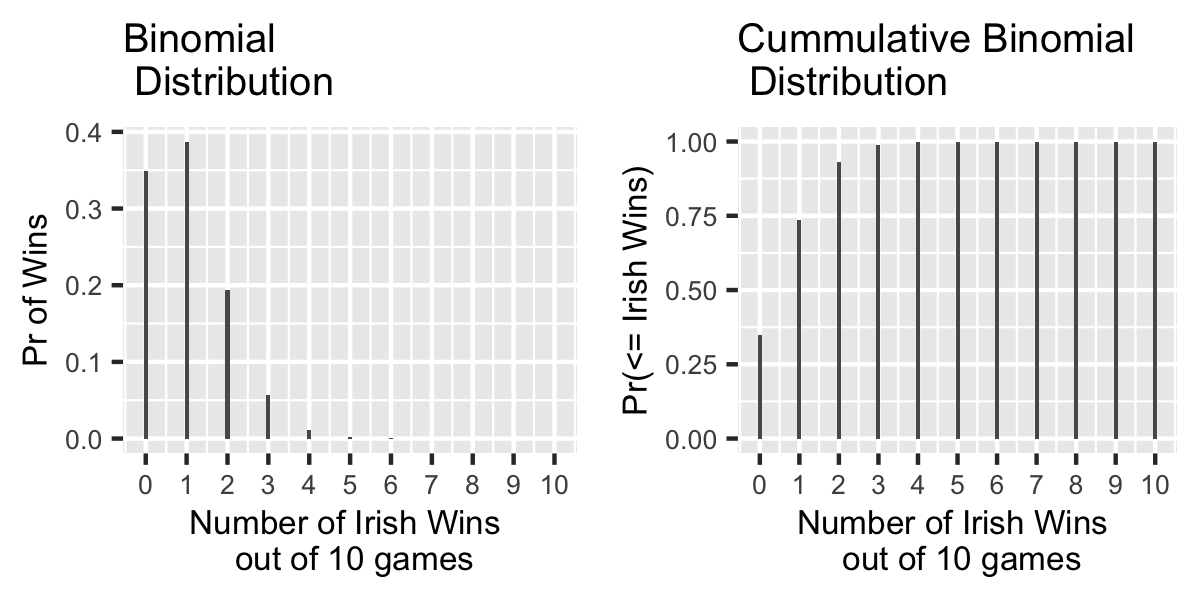
\includegraphics[width=\textwidth]{Figures/Distributions/Binomial.png}
\end{subbox}

\begin{subbox}{subbox}{Geometric Distribution}
\tiny
The formula for the Geometric distribution is:
\[\Pr(k)=q^{(k-1)}p, \ \ k=1,2,... \]
	\[E[k]=\frac{1}{p}, \ \ \ Var[k]=\frac{q}{p^2}.\]
    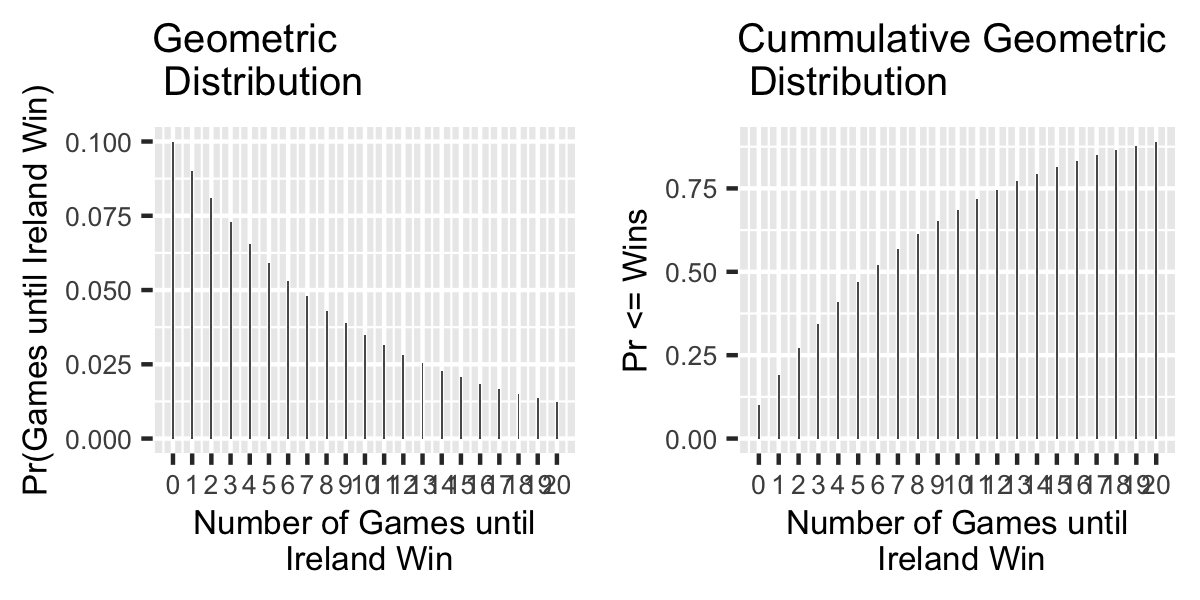
\includegraphics[width=\textwidth]{Figures/Distributions/Geometric.png}
\end{subbox}
\end{textbox}
%%% DISCRETE DISTRIBUTION
\begin{textbox}{Discrete Distribution}

\begin{subbox}{subbox}{Poisson Distribution}
	\tiny
	The formula for the Poisson distribution is:
	\[\Pr(k)=\frac{\lambda^ke^{-\lambda}}{k!}, \ \ k=0,1,2,... \]
	\[E[k]=\lambda, \ \ \ Var[k]=\lambda. \]

    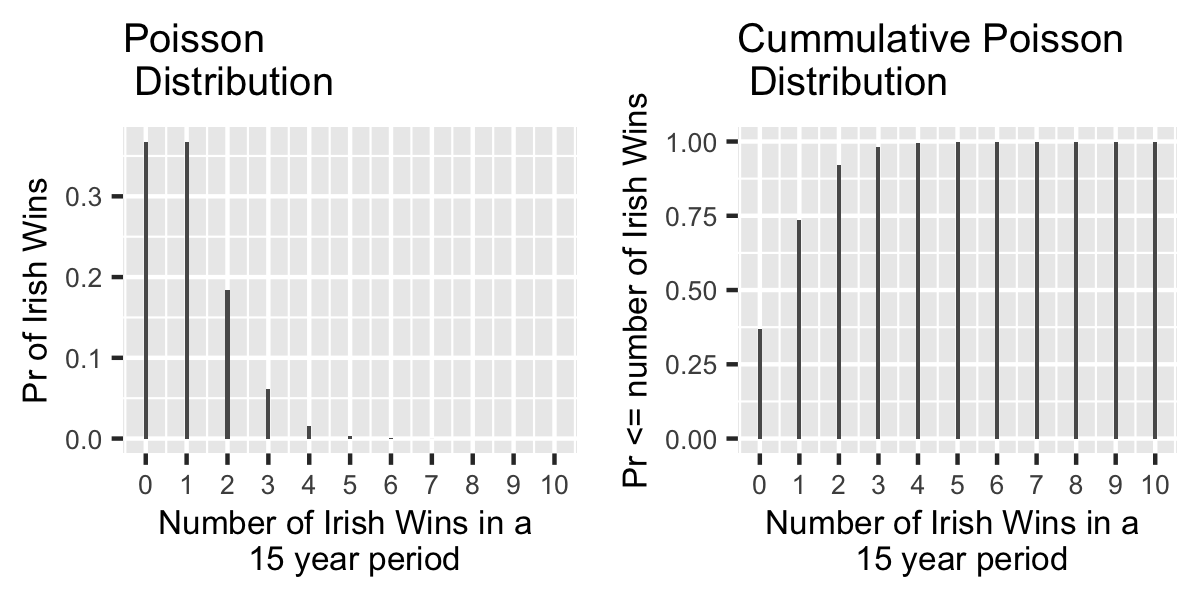
\includegraphics[width=\textwidth]{Figures/Distributions/Poisson.png}
\end{subbox}

\end{textbox}
\begin{textbox}{Continuous Distribution}
\begin{subbox}{subbox}{Normal Distribution}
    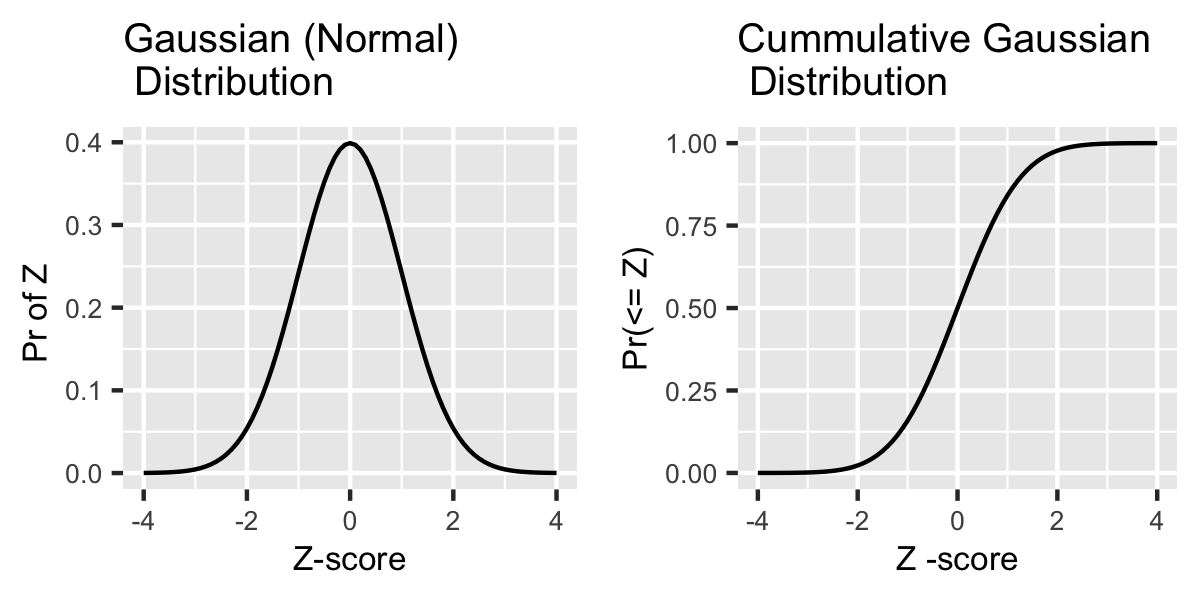
\includegraphics[width=\textwidth]{Figures/Distributions/Normal.png}
\end{subbox}
\begin{subbox}{subbox}{Confidence Intervals}
\begin{center}
\tiny
    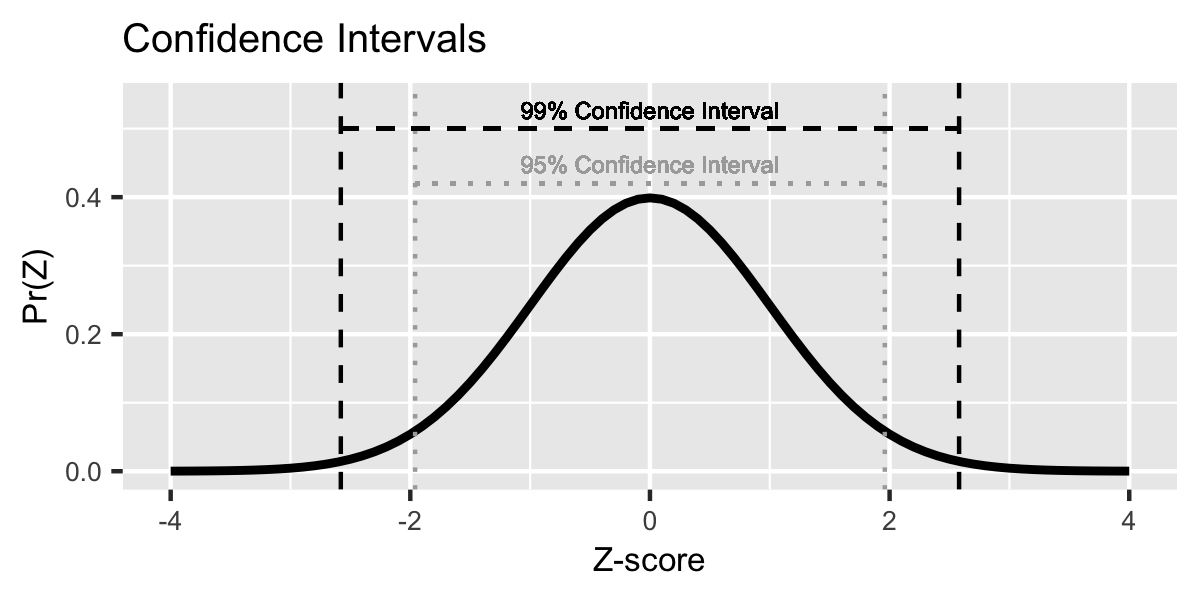
\includegraphics[width=\textwidth]{Figures/Distributions/CI_Normal.png}
\end{center}
\end{subbox}

\end{textbox}
\begin{textbox}{Hypothesis Testing}
Five steps for Hypothesis testings
\begin{enumerate}
\item  State the Null Hypothesis $H_0$;
\item  State an Alternative Hypothesis $H_{ alpha}$;
\item  Calculate a Test Statistic (see below);
\item  Calculate a p-value and/or set a rejection region;
\item  State your conclusions.
\end{enumerate}
\end{textbox}
\begin{textbox}{z-test}
\begin{subbox}{subbox}{Continuous Data}
The test statistic is given by
\[Z=\frac{\bar{x}-\mu}{\frac{\sigma}{\sqrt{n}}} \sim N(0,1), \]
where $\bar{x}$ is the observed mean, $\mu$ is the historical mean, $\sigma$ is the standard deviation and $n$ is the number of observations.

\begin{subbox}{subbox}{Do supplements make you faster? }
\tiny
The effect of a food supplements on the response time in rats is of interest to a biologist. They have established that the normal response time of rats is $\mu=1.2$ seconds. The $n=100$ rats were given a new food supplements. The following summary statistics were recorded from the data $\bar{x}=1.05$ and $\sigma= 0.5$ seconds
\begin{enumerate}
    \item The rats in the study are the same as normal rats,  $H_0 : \bar{x}=1.2$. 
\item The rats are different, $H_\alpha:\bar{x}\not= 1.2$.
\item Calculate a Test Statistic $Z=\frac{1.05-1.2}{\frac{0.5}{\sqrt{100}}}=-3 $
\item Reject the Null hypothesis $h_0$ if $Z<-1.96$ and $Z>1.96$
\item The data suggests that rats are faster with the new food.
\end{enumerate}


\end{subbox}
\end{subbox}
\begin{subbox}{subbox}{Proportional Data}
The test statistic is given by
\[z=\frac{\hat{p}-p}{\sqrt{\frac{pq}{n}}} \sim N(0,1). \]
where $\hat{p}$ is the observed proportion, $p$ is the historical proportion, $q$ is the complement $q=1-p$,  and $n$ is the number of observations.
\end{subbox}
\end{textbox}
\begin{textbox}{t-test}
\begin{subbox}{subbox}{paired t-test}

 The test statistic is given by  \[ t={\frac {{\bar {x}}-{\bar \mu_0}}{\frac{s}{\sqrt n}}} \sim t_{\alpha,df}\]
where $\bar{x}$ is the observed mean, $\mu_0$ is the null mean, $s$ is the standard deviation and $n$ is the number of observations.
\end{subbox}
\begin{subbox}{subbox}{unpaired t-test}
The test statistic is given by
\[ t={\frac {{\bar {x}}_{1}-{\bar {x}}_{2}}{s_{p}{\sqrt {\frac {1}{n_1}+\frac{1}{n_2}}}}} \sim t_{\alpha,df}\]
 where
$s_{p}={\sqrt{\frac {s_{x_{1}}^{2}+s_{x_{2}}^{2}}{2}}}$ is the pooled sample standard deviation, $\bar{x}_1$ and $\bar{x}_2$ are the sample means, $n_1$ and $n_2$ are the sample sizes.
\end{subbox}
\end{textbox}
\begin{textbox}{$\chi^2$ Independence test}
The test statistic to test if data are independent of group is given by:
   	\[\chi^2_{Ind}=\sum \frac{(O-E)^2}{E} \sim \chi^2_{(r-1)(c-1)}.\]
where $O$ is the observed data, $E$ is the expected data if independent, $r$ is the number of rows and $c$ is the number of columns.\\
\begin{subbox}{subbox}{Does ice-cream flavour matter?}
\tiny
An ice-cream company had 500 people sample one of three different ice-cream flavours and asked them to say whether they liked or disliked the ice-cream. 
\begin{center}
\begin{tabular}{|l|r|r|r|}
\hline
&Vanilla&Chocolate& Strawberry\\
\hline
Liked&130&170&100\\
\hline
Disliked&20&30&50\\
\hline
\end{tabular}
\end{center}
The $\chi^2_{Ind}$ independence test could be used to determine if the enjoyment of the ice-cream depends on the flavour.\\
\end{subbox}
\end{textbox}
\begin{textbox}{$\chi^2$ Goodness of Fit}
The test statistic to test if data come from a specific distribution is given by:
\[\chi^2_{GoF}=\sum \frac{(O-E)^2}{E} \sim\chi^2_{k-1},\]
where $O$ is the observed data, $E$ is the expected data from a chosen distribution and $k$ is the number of observation bins.
\begin{subbox}{subbox}{Does it fit?}
\tiny
The $\chi^2_{GoF}$ can test if the observed distribution of the height of Dutch people (grey) fits the expected distribution of heights (dark grey).

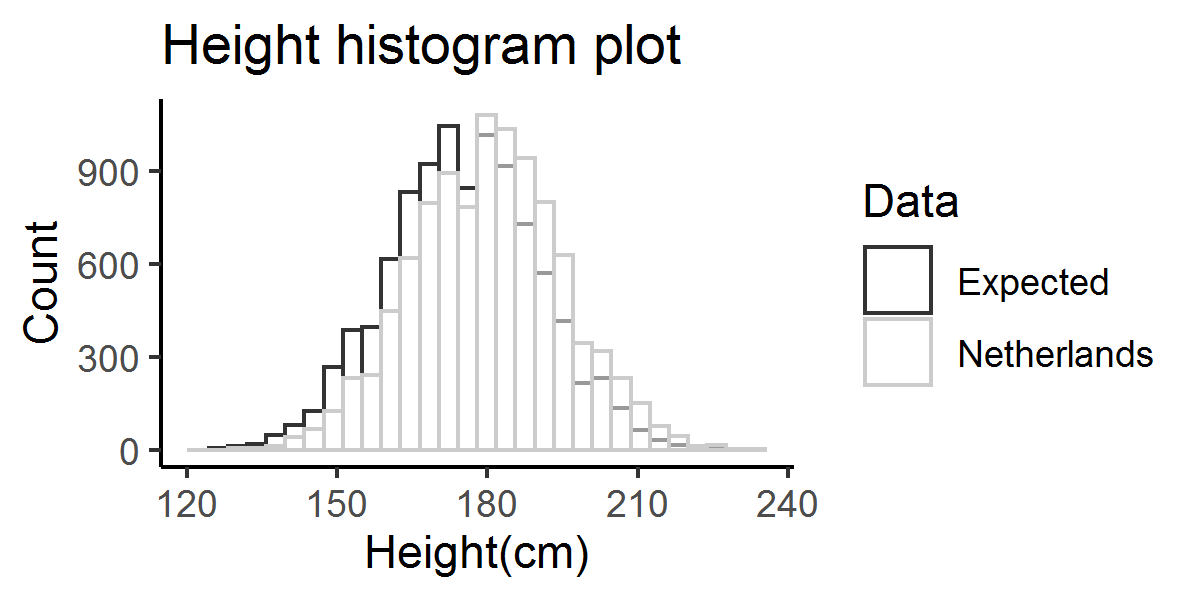
\includegraphics[width=\textwidth]{Figures/Distributions/GoF.png}
\end{subbox}
\end{textbox}

\begin{textbox}{Linear Regression}

A linear regression is used to model a linear relationship of the dependent variable $y$ and the regressors $x_1$, $x_2$, ...
	\[  y=\beta_0+\beta_1 x_{1} +\beta_2 x_{2}+..., \]
	where $\beta_0$, $\beta_1$ are the slopes of the regressors.

\begin{subbox}{subbox}{Height Prediction}
\tiny
A simple linear regression (correlation) is used to predict the height of 744 children $y$ using the height of their parent $x$, 
\[  y=\beta_0+\beta_1 x.\]
The plot below shows the fit of the model:
\begin{center}
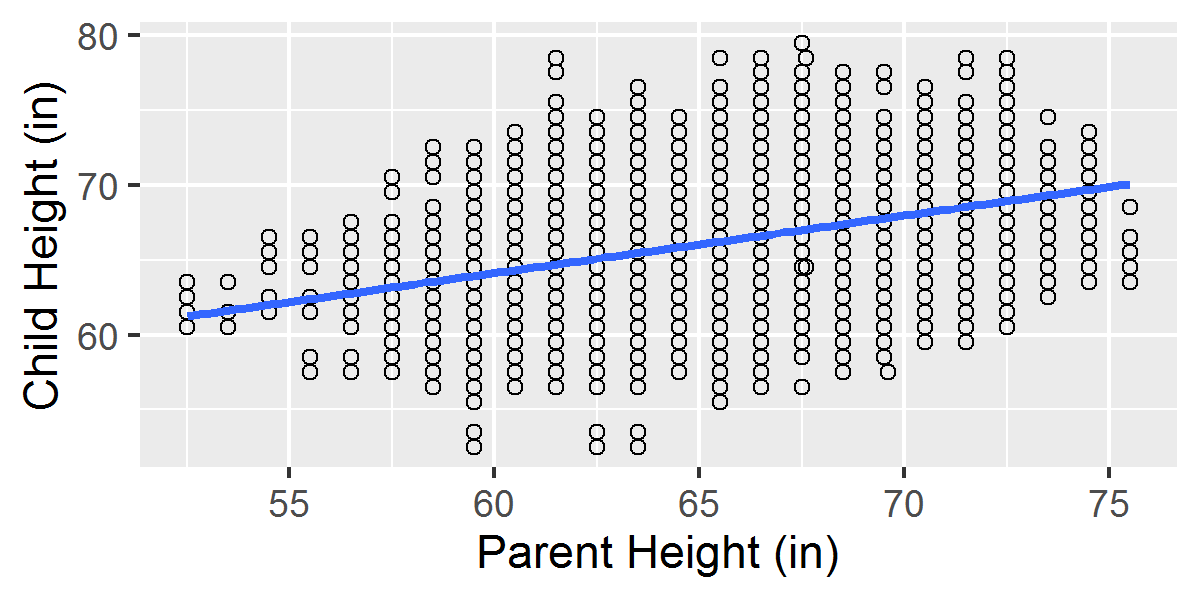
\includegraphics[width=\textwidth]{Figures/Regression/Linear_Regression.png}
\end{center}
The parents' height $x$ explained $12.7\%$ of the children's' height $y$.
\end{subbox}
\end{textbox}
\begin{textbox}{ANalysis Of VAriance (ANOVA)}
A one-way ANOVA logistic regression is used to compare more than one groups.
The general formula for the ANOVA is 
	\[  x_{ij}=\bar{x}+a_j+\varepsilon_{ij}, \]
where $x_{ij}$ is each element, $\bar{x}$ is the overall average, $a_j$ is the group different and $\varepsilon_{ij}$ are the residuals.

\begin{subbox}{subbox}{Comparison between three groups}
\tiny
Data from three different groups (A, B, C) was observed and compared using an ANOVA.
The plot below shows the box-plots for the groups and the post-hoc comparion:
\begin{center}
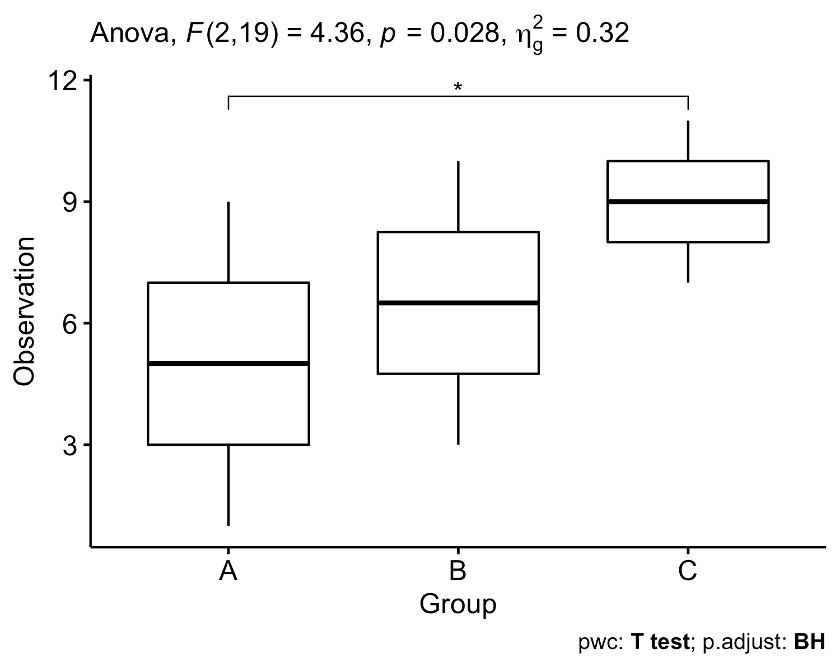
\includegraphics[width=\textwidth]{Figures/ANOVA/Picture1.png}
\end{center}
The ANOVA revealed a significant difference between the groups and the post hoc showed it was driven by differences between groups A and C.
\end{subbox}
\end{textbox}
\begin{textbox}{Bibliography}
\begin{enumerate}
\item 
Devore \& Peck  - Statistics: The exploration and analysis of data (2011)
\item James, G., Witten, D., Hastie, T., \& Tibshirani, R. (2013). An introduction to statistical learning (Vol. 112, p. 18). New York: springer. 
\href{https://www.statlearning.com}{book website}
\item Poldrack R. Statistical Thinking in the 21st Century 2020 \href{https://statsthinking21.github.io/statsthinking21-core-site/index.html}{website}
\item
Gareth, J., et al. - An introduction to statistical learning. Vol. 112. New York: Springer, 2013.
\item
Fry, H. - Hello World: How to be Human in the Age of the Machine, Doubleday, 2018
\item Butler, J. S., \href{https://github.com/john-s-butler-dit/Probability_and_Statistical_Inference}{Course GitHub Repository}  

\end{enumerate}


\end{textbox}

\end{multicols}

\end{document}
